\documentclass[border=5mm]{standalone}
\usepackage{tikz}
\usepackage{tikz-qtree}

\begin{document}
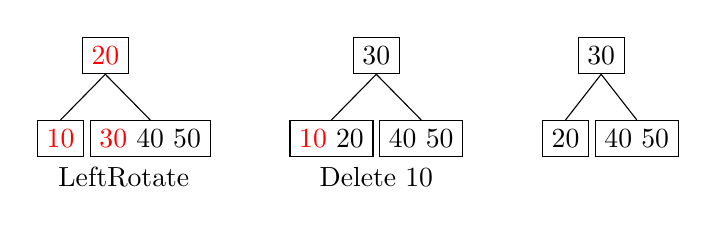
\begin{tikzpicture}[every tree node/.style={align=center}]
    \matrix[row sep=1cm, column sep=1cm] {
    \Tree
    [.\node[draw, rectangle]{\textcolor{red}{20}};
    [.\node[draw, rectangle]{\textcolor{red}{10}}; ]
    [.\node[draw, rectangle]{\textcolor{red}{30} 40 50};    ]
    ];
    \node[below] at (current bounding box.south) {LeftRotate};
    &
    \Tree
    [.\node[draw, rectangle]{30};
    [.\node[draw, rectangle]{\textcolor{red}{10} 20}; ]
    [.\node[draw, rectangle]{40 50};    ]
    ]; 
    \node[below] at (current bounding box.south) {Delete 10};
    &
    \Tree
    [.\node[draw, rectangle]{30};
    [.\node[draw, rectangle]{20}; ]
    [.\node[draw, rectangle]{40 50};    ]
    ]; \\
    };

\end{tikzpicture}
\end{document}
